\chapter{Introduction}
\marginnote{This may exist as another name, but I don't think so, and it really should be called luck.  A Rose by the name of Rosaceae would be lost.}

The point of these notes is to introduce an idea of ``luck'' that connects mathematical probability with the everyday notion.

As a motivating problem, imagine walking along the beach and asking a random person to toss a tennis ball so that it lands in the sand.  The probability that it lands at some point would depend on the habits of the thrower and the details of the beach, but we can summarize this as some probability distribution, $p(x)=\rho(x) dx$, where $x\in\R^2$ is a suitable coordinate system for the beach in question.  It would almost certainly not be a uniform distribution, and it would almost certainly not be particularly concentrated.

Traditional probability feels uncomfortable here.  The chances of the ball landing at a given point is zero\marginnote{For a continuous probablity distribution such as this, the chance of the ball landing in some small area $dx$ near $x$ is $p(x)=\rho(x) dx$.  But the ball lands at a point, so $dx$ is zero, so the probablity $p(x)=\rho(x) dx$ is zero.}, and so miraculous.  Yet anyone watching this process would only occasionaly be surprized by the outcome.

As common (and mundane, not miraculous) such situations are, the language of statistics seems to have difficulty with the notion.  Nor is it limited to continuous cases, just when there are a lot of possible outcomes.  Such examples lead to non-zero but very small probabilities.\marginnote{The real motivation of this came from the space of passwords a person might choose from, which is an effectively infinite discrete space.}

To distinguish from the more general notion of luck, note that that there is no extrinsic value on an outcome.  To say something is ``lucky'' often means there is some value (different from the probability) associated with outcomes.  However, outcomes that are the most valuable are often the least probable, and outcomes of equal probability ought to be equally lucky.  In the most extreme case of all equally probable outcomes (uniform probability), every outcome should have a luck of $\frac{1}{2}$.  

These observations lead to the following definition of luck:
\begin{quote}
The luck $L(x)$ of an outcome $x$ is the probability of getting any outcome $y$ that is more probable than $x$, plus one-half the probability of getting any outcome $y$ that is equally probable to $x$.
\end{quote}

From the perspective of discussing luck, it is convenient to have few sets: $\Omega(x)$, the outcomes more likely than $x$, and $\omega(x)$, the outcomes equally likely to $x$.

\begin{definition}{Omega.}  $\Omega(x)$ is set of outcomes more likely than $x$:
\begin{equation}
\Omega(x) = \left\{ y \mid p(y)>p(x) \right\} \,.
\end{equation}
We define $|\Omega(x)|$ as the probability an outcome is in $\Omega(x)$,
$|\Omega(x)| = P(y\in\Omega(x))$.  In the discrete case, this is
\begin{equation}
|\Omega(x)| = \sum_{y \in \Omega(x)} p(y),
\end{equation}
and, in the continuous case,
\begin{equation}
|\Omega(x)| = \int_{\Omega(x)} \rho(y)\,dy \,.
\end{equation}
\end{definition}

\begin{definition}{omega.}\marginnote{For the tyical case of many outcomes with different probabilities, $|\omega(x)|$ is small.  For example, $|\omega(x)|=0$ for any multivariate normal distribution.}
$\omega(x)$ is the set of outcomes equally likley to $x$:
\begin{equation}
\omega(x) = \left\{ y \mid p(y)=p(x) \right\} \,.
\end{equation}
Similar to $\Omega(x)$, we define $|\omega(x)|$ as the probability an outcome is in $\omega(x)$,
$|\omega(x)| = P(y\in\omega(x))$.  

In the discrete case, this is
\begin{equation}
|\omega(x)| = \sum_{y \in \omega(x)} p(y),
\end{equation}
and, in the continuous case,
\begin{equation}
|\omega(x)| = \int_{\omega(x)} \rho(y)\,dy \,.
\end{equation}
\end{definition}

With these definitions in place, we define luck mathematically as follows:
\begin{definition}{Luck.}  The luck of an outcome is the probability getting any more likely outcome, plus half the probability of getting any equally likely outcome:
\begin{equation}
L(x)=|\Omega(x)| + \frac{1}{2} |\omega(x)| \,.
\end{equation}
\end{definition}

\subsection{Properties of Luck.}
\begin{itemize}
\item Range of luck. $0 \leq L(x) \leq 1$.  This ranges from no luck to perfect luck.
\item Lucky outcomes. If $L(x)$ is close to 1, then $p(x)$ is comparatively small, and most outcomes would have a higher probability (you are lucky).  
\item Unlucky outcomes. If $L(x)$ is close to 0, then $p(x)$ is comparatively large, and most outcomes would have a lower probability (you are unlucky).
\item Luck on average. $E(L)=\frac{1}{2}$.  On average, luck is always 50:50.
\end{itemize}

We are interested in cases which have many possible outcomes with low but somewhat different probabilities (like the tennis ball on the beach).  If the space is well divided (so $\max |\omega|=\max_{x}|\omega(x)|$ is small), then there are other interesting properties of luck:\marginnote{In particular $|\omega(x)|=0$ for the normal, exponential, beta, and gamma distributions.  As a worst-case counterexample, the flattest distribution is the uniform distribution, for which $|\omega(x)|=1$.}

For the kind of distributions with small $\max |\omega|$, luck is a very uniformizing transformation (there can be no better, actually).  If it were exactly uniform, the following would be correct with $\varepsilon=0$.  There is no other functional of the probability space alone with smaller error bounds:
\begin{itemize}
\item For any $f: [0,1] \rightarrow \mathbb{R}$ with bounded second derivative, $E(f(L))=\int_0^1 f(L) dL-\varepsilon$, where $|\varepsilon| \leq \max|f''| \cdot \max |\omega|^2 / 24$.
\item For $p \geq 2$, $E(L^p)=1/(p+1)-\varepsilon$, $0 \leq \varepsilon \leq p \cdot (p-1) \max |\omega|^2/24$.
\item For $0 \leq a \leq b \leq 1$, $E(L \in [a,b])=b-a - \varepsilon$, $|\varepsilon| \leq \max |\omega|$.
\end{itemize}
The proofs of these come from the midpoint integration rule and thinking about the general case for figure~\ref{fig:arrange} below.

\begin{example}{Coins.}
Suppose we toss 8 fair coins.  The probability of getting exactly $x$ heads out of 8 tosses is given by the binomial distribution
\begin{equation}
p(x)=\frac{8!}{x!(8-x)!}\left(\frac{1}{2}\right)^8 \,.
\end{equation}
What is the luck associated with this distribution?
\begin{table}
\caption{This is arranged in increasing luck (which is decreasing probability). Getting exactly $x=4$ heads is unlucky, requiring only $L=14\%$ luck, while getting $x=0$ or $x=8$ heads is almost $100\%$ luck.}
\begin{tabular}{|c|S[table-format=2.4]|c|S[table-format=2.4]|c|S[table-format=2.4]|c|S[table-format=2.4]|S[table-format=2.4]|}
\multicolumn{1}{c}{$x$} &
\multicolumn{1}{c}{$p(x)$} &
\multicolumn{1}{c}{$\Omega(x)$} &
\multicolumn{1}{c}{$|\Omega(x)|$} &
\multicolumn{1}{c}{$\omega(x)$} &
\multicolumn{1}{c}{$|\omega(x)|$} &
\multicolumn{1}{c}{$L(x)$} \\
\hline
     4 & 0.2734 &  \{\} & 0.0000 & \{4\} & 0.2734 & 0.1367 \\
3 or 5 & 0.2188 & \{4\} & 0.2734 & \{3,5\} & 0.4375 & 0.4922 \\
2 or 6 & 0.1094 & \{3,4,5\} & 0.7109 & \{2,6\} & 0.2188 & 0.8203 \\
1 or 7 & 0.0313 & \{2,3,4,5,6\} & 0.9297 & \{1,7\} & 0.0625 & 0.9609 \\
0 or 8 & 0.0039 & \{1,2,3,4,5,6,7\} & 0.9922 & \{0,8\} & 0.0078 & 0.9961 \\
\hline
\end{tabular}
\end{table}
\begin{figure}
\begin{center}
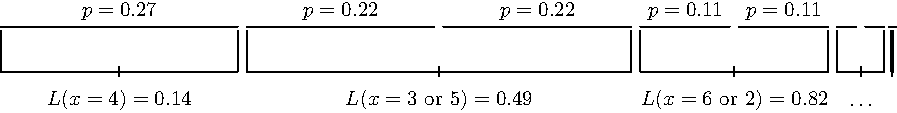
\includegraphics[width=1.00\linewidth]{graphics/arrange.pdf}
\end{center}
\caption{\label{fig:arrange}Luck to get $x$ heads on $8$ fair coins.  After the probabilities are arranged in decreasing order on the unit interval, $L(x)$ is the center point of equally probable outcomes.}
\label{fig:arrange}
\end{figure}

Luck on average is $\frac{1}{2}$:
\marginnote{For any distribution, $E(L)=\frac{1}{2}$.}
\begin{equation}
E(L)=\sum_{x=0}^8 p(x) \cdot L(x) = \frac{1}{2} \,.
\end{equation}

The second moment should be close to $\frac{1}{3}$:
\marginnote{For any distribution, $E(L^2)=\frac{1}{3}-\varepsilon$, with $0 \leq \varepsilon \leq \max |\omega|^2/12$.

For the coin distribution, the bound is $0 \leq \varepsilon \leq 0.016$, and the actual error $\varepsilon=0.0096$.}
\begin{equation}
E(L^2)=\sum_{x=0}^8 p(x) \cdot L(x)^2 = \frac{1}{3} - 0.0096
\end{equation}

The probability luck is in the middle half is about $\frac{1}{2}$:
\marginnote{For any distribution, $E(L \in [a,b]) = b-a+\varepsilon$, with $|\varepsilon|\leq \max |\omega|$.

For the coin distribution and $[a,b]=[\frac{1}{4},\frac{3}{4}]$, $E(L \in [a,b])=\frac{1}{2}+\varepsilon$ with $|\varepsilon|\leq 0.4375$ as the (poor) error bound, and the actual error of $\varepsilon=-0.0625$}
\begin{equation}
\begin{split}
E(L \in [\frac{1}{4},\frac{3}{4}]) &= \sum_{x=0}^8 p(x) \cdot 
\left\{ \begin{array}{cl} 1 & \text{if $L(x) \in [\frac{1}{4},\frac{3}{4}]$} \\
                          0 & \text{otherwise} 
\end{array} \right\} \\
&= \frac{1}{2} - 0.0625 \,.
\end{split}
\end{equation}
\end{example}
\begin{example}{Normal.}  This is a special case of the multivariate normal we cover in the next section, but working out the details for the one-dimensional case can be illuminating.  We define the one-dimensional normal distribution with mean $\mu$ and variance $\Sigma$ as
\begin{align}
P_{\text{normal}}(x;\mu,\Sigma) &= \frac{e^{-\frac{(x-\mu)^2}{2\Sigma}}}{\sqrt{2\pi\Sigma}} \,,\\
\intertext{where}
\mu &= E(x)\,,\\
\intertext{and}
\Sigma &= E((x-\mu)^2) \,.
\end{align}

First note that $\Omega(x)$ is the open the interval between $x$ and $x$ reflected around $\mu$:
\begin{equation}
\Omega(x)=(\min(x,2\mu-x),\max(x,2\mu-x)) \,,
\end{equation}
and $\omega(x)$ is the endpoints of that interval:
\begin{equation}
\omega(x)=\{x,2\mu-x\} \,.
\end{equation}

Since the 1-dimensional normal distribution is a continuous distribution and $\omega(x)$ is a finite set, $|\omega(x)|=0$, i.e.,
\begin{equation}
|\omega(x)|=\int_{\omega(x)} P_{\text{normal}}(y;\mu,\Sigma) \, dy = 0 \,.
\end{equation}
This means all the luck properties are exact (the error terms are zero), and the $\frac{1}{2}|\omega(x)|$ contributes nothing to the luck of an outcome.

What remains is to calculate luck,
\begin{equation}
L(x)=\int_{\Omega(x)} P_{\text{normal}}(y;\mu,\Sigma) \, dy \,.
\end{equation}
Changing variables to the normalized $z$-score: $z=\sqrt{\Sigma^{-1}}(x-\mu)$, this can be rewritten as
\begin{equation}
L(x)=\int_{-R}^{R} P_{\text{normal}}(y,0,1) \, dy \,,
\end{equation}
where
\begin{equation}
R=|\sqrt{\Sigma^{-1}}(x-\mu)| \,.
\end{equation}

Using $\erf(x)$, defined as\marginnote{$\erf(x)$ is a normalized integral of the $P_{\text{normal}}(x;\mu=0,\Sigma=1/2)$ so that $\erf(0)=0$ and $\erf(\pm \infty)=\pm 1$.}
\begin{equation}
\erf(x) = \frac{2}{\sqrt{\pi}} \int_0^x e^{-y^2} \, dy \,, 
\end{equation}
the luck of an outcome can be written as
\begin{equation}
\label{eq:normal-1d-luck}
L(x)=\erf\left|\frac{x-\mu}{\sqrt{2\Sigma}} \right| \,.
\end{equation}

In the next chapter, where we address the more general multivariate normal case, we obtain the approximation,
\begin{equation}
\label{eq:approx-normal-1d-luck}
L(x) \approx \frac{1}{2} \left[ 1+\erf\left(\left|\frac{x-\mu}{\sqrt{\Sigma}} \right|-\sqrt{\frac{1}{2}}\right)\right] \,.
\end{equation}
Figure~\ref{fig:normal1} compares the exact and approximate result in the 1-d case.

\begin{figure}
\begin{center}
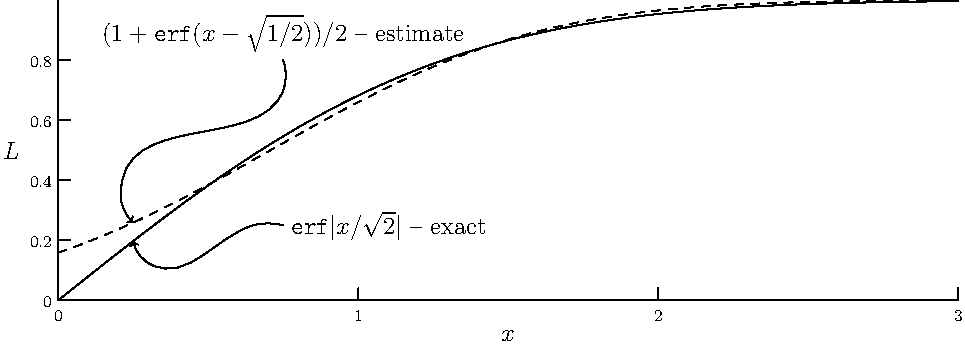
\includegraphics[width=0.75\linewidth]{graphics/normal1.pdf}
\end{center}
\caption{Exact (solid, equation~\ref{eq:normal-1d-luck}) vs approximate (dashed, equation~\ref{eq:approx-normal-1d-luck}) luck for 1-d normal distribution.}
\label{fig:normal1}
\end{figure}
\end{example}

\section{Asymmetric distributions and $p$-values vs. luck.}
For symmetric or monotonic one dimensional continuous distributions, the connection between luck and $p$-values can be pretty simple.  However, the relation between $p$ and $L$ can be complex.  Figure~\ref{fig:chi2} shows the $p$-values vs luck for $\rchi^2(x,k)$ for $k=4$ distribution.

\begin{figure}
\begin{center}
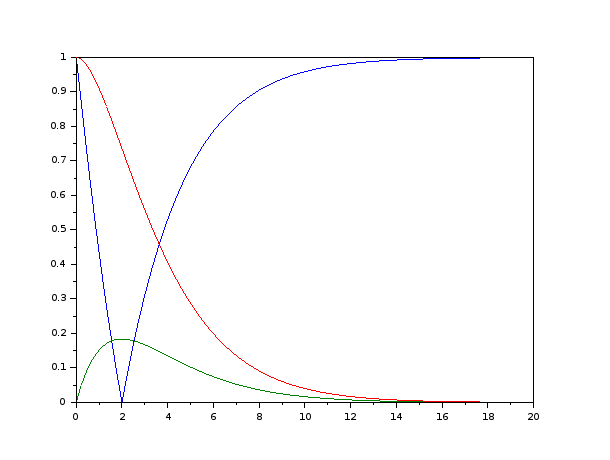
\includegraphics[width=0.75\linewidth]{img/chi2.png}
\end{center}
\caption{$p$-value (red) vs $L$ (blue) for the $\rchi^2$ distribution for $k=4$ (in green).  There is no simple relationship between $L$ and $p$.}
\label{fig:chi2}
\end{figure}
In Chapter~\ref{chap:chi2}, we show a good approximation for large $k$ is
\begin{equation}
  L[\rchi^2_k](x)\approx \erf(\left|\sqrt{x}-\sqrt{k-2}\right|) \,.
\end{equation}

\section{Summary}
\begin{itemize}
\item Luck has a natural definition of
  \begin{equation*}
    \begin{split}
    \Luck(x) = &\Prob(\text{anything more likely than $x$}) \\
    & + \frac{1}{2} \Prob(\text{$x$ or anything equally likely to $x$}) \,.
    \end{split}
    \end{equation*}
  \item Luck ranges from $0$ (no luck) to $1$ (perfect luck).
  \item The expected value of luck is always exactly $1/2$.
  \item Luck is very nearly uniform, and there is no better map to a uniform distribution for a general probability distribution. 
  \item For the 1-d normal distribution with mean $\mu$ and standard deviation $\sigma$:
    \begin{equation*}
L[{\cal N}_{1d}(\cdot;\mu,\sigma^2)](x)=\erf \left|\frac{x-\mu}{\sqrt{2\Sigma}} \right| \,.      
    \end{equation*}
  \item For the 1-d $\rchi^2_k$ distribution, there is no simple form, but for large $k$:
    \begin{equation*}
      L[\rchi^2_k](x) \approx \erf \left| \sqrt{x}-\sqrt{k-2} \right| \,.
    \end{equation*}
\end{itemize}

\section{Exercises}
\begin{enumerate}
\item \label{q:intro-coin} Take the maximum of two fair coin flips (0 or 1), so $\Prob(\max = 0)=1/4$ and $\Prob(\max = 1)=3/4$.  What is the luck of each outcome?
\item \label{q:intro-coins} Take 3 independent trials like problem \ref{q:intro-coin}.  Note there are $2^3$ outcomes but only 3 distinct probabilites.  Show that
  \begin{gather*}
    L((0,0,0))=\frac{27}{128} \approx 0.2109 \\
    L((1,0,0))=L((0,1,0))=L((0,0,1))=\frac{81}{128} \approx 0.6328 \\
    L((0,1,1))=L((1,0,1))=L((1,1,0))=\frac{117}{128} \approx 0.9141 \\
    L((1,1,1))=\frac{127}{128} \approx 0.9922
  \end{gather*}
\item \label{q:intro-coin-test} Use a strong random number generator (like {\tt random.org}) to make 3 independent trials for the maximum of 2 fair coin tosses.  What is the luck of the outcome?
\item \label{q:intro-exp} Now write down what feels like a random sequence of six zeros and ones --- don't think too hard about it!  Use these in pairs like problem \ref{q:intro-coin-test}.  What was the luck of this outcome?
\item Calculate the luck $L(x)$ for the exponential distribution $p(x)=\lambda \exp(-\lambda x)$ for $x\geq 0$ and $\lambda > 0$.

\item In {\em Rosencrantz and Guildenstern Are Dead}, Guildenstern tosses 85 heads in a row at the beginning of the play.  Taken as a sequence of fair coin tosses, why is Guildenstern luck 1/2?

\item Ignoring the last coin toss, group the 84 heads as 42 experiment pairs like (\ref{q:intro-coin}).  Show from this perspective Guildenstern is unlucky:
  \begin{equation*}
    L=\frac{109418989131512359209}{38685626227668133590597632} \approx 2.828 \times 10^{-6} \,.
  \end{equation*}
\item Now consider the minimum-of-pairs problem for the 42 head-pairs.  Show that for this problem Guildenstern insanely lucky:
  \begin{equation*}  
  L=1-2^{-85} \approx 1-2.585\times 10^{-26}
  \end{equation*}
\end{enumerate}
